\documentclass[../Matematyka.tex]{subfiles}

\begin{document}
    \section{Elementy kombinatoryki i teorii mnogości}

    \subsection{Działania na zbiorach}

    \subsubsection*{Suma}
    \[C = A \cup B\]

    \begin{figure}[H]
        \centering
        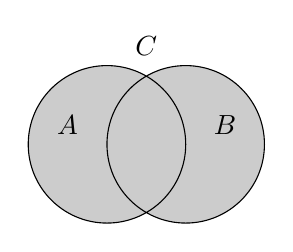
\begin{tikzpicture}[fill=black!20]
            \fill (-0.5,0) circle (1);
            \fill (0.5,0) circle (1);
            % outline
            \draw (-0.5,0) circle (1) (-1,0)  node [text=black,above] {$A$}
                (0.5,0) circle (1) (1,0)  node [text=black,above] {$B$}
                (0,1)  node [text=black,above] {$C$};
        \end{tikzpicture}
    \end{figure}

    \subsubsection*{Iloczyn}
    \[D = A \cap B\]

    \begin{figure}[H]
        \centering
        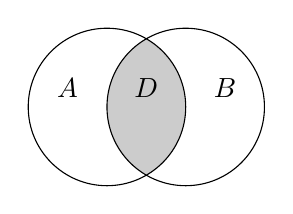
\begin{tikzpicture}[fill=black!20]
            \begin{scope}[even odd rule]
                \clip (-1.5,-1) rectangle (1.5,1) 
                    (-0.5,0) circle (1) 
                    (0.5,0) circle (1);
                \fill (-0.5,0) circle (1);
                \fill (0.5,0) circle (1);
            \end{scope}
            % outline
            \draw (-0.5,0) circle (1) (-1,0)  node [text=black,above] {$A$}
                (0.5,0) circle (1) (1,0)  node [text=black,above] {$B$}
                (0,0)  node [text=black,above] {$D$};
        \end{tikzpicture}
    \end{figure}

    \subsubsection*{Różnica}
    \[E = A \setminus B\]

    \begin{figure}[H]
        \centering
        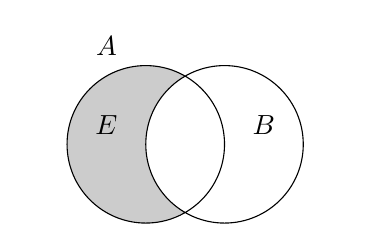
\begin{tikzpicture}[fill=black!20]
            \begin{scope}
                \clip (-2,-1) rectangle (2,1) 
                    (0.5,0) circle (1);
                \fill (-0.5,0) circle (1);
            \end{scope}
            % outline
            \draw (-0.5,0) circle (1) (-1,1)  node [text=black,above] {$A$}
                (-1,0)  node [text=black,above] {$E$}
                (0.5,0) circle (1) (1,0)  node [text=black,above] {$B$};
        \end{tikzpicture}
    \end{figure}

    \subsubsection*{Dopełnienie zbioru}
    \[A` = X \setminus A\]

    \begin{figure}[H]
        \centering
        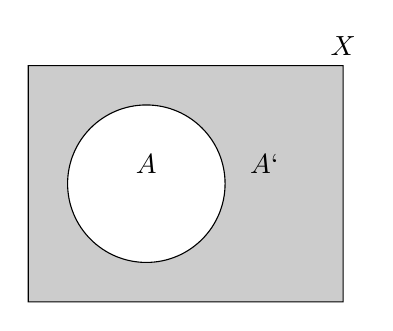
\begin{tikzpicture}[fill=black!20]
            \begin{scope}
                \clip (-0.5,0) circle (1)
                    (-2,-1.5) rectangle (2,1.5);
                \fill (-2,-1.5) rectangle (2,1.5);
            \end{scope}
            % outline
            \draw (-0.5,0) circle (1) (-0.5,0)  node [text=black,above] {$A$}
                (-2,-1.5) rectangle (2,1.5) node [text=black,above] {$X$}
                (1,0) node [text=black,above] {$A`$};
        \end{tikzpicture}
    \end{figure}

    \newpage
    \subsection{Iloczyn kartezjański}
    \[A \times B = \{(a, b) : a \in A \; \text{i} \; b \in B\}\]

    \[A = \{a, b, c\} \qquad B = \{1, 2\}\]
    \[A \times B = \{(a,1)(a,2)(b,1)(b,2)(c,1)(c,2)\}\]

    Oznaczenie: \(|X|\) - ilość elementów

    Tw. \(|A \times B| = |A| \cdot |B|\)

    \(\mathbb{R}\) - zbiór liczb rzeczywistych (prosta liczbowa)\par
    \(\mathbb{R}^2 = \mathbb{R} \times \mathbb{R} = \{(x,y) : x \in \mathbb{R} \; \text{i} \; y \in \mathbb{R}\}\) - płaszczyzna\par
    \(\mathbb{R}^n \) - przestrzeń \(n\) wymiarowa

    \subsection{Kombinatoryka}

    \subsubsection{Silnia}
    \(n!\) - \(n\) silnia \(\qquad n \in \mathbb{N}_0\)

    \begin{displaymath}
        n! =
        \begin{cases}
            1, & \quad n = 0 \lor n = 1 \\
            1 \cdot 2 \cdot \ldots \cdot n, & \quad n > 1
        \end{cases}
    \end{displaymath}

    \[n! = (n - 1)! \cdot n, \quad n \in \mathbb{N}\]

    Def. Permutacja skończonego zbirou \(A\) to ciąg wszystkich elementów zbioru \(A\).\par
    Tw. Ilość wszystkich permutacji zbioru \(n\)-elementowego wynosi \(n!\).

    \subsubsection{Symbol Newtona}

    \begin{align*}
        \binom{n}{k} = 
        \frac{n!}{k!(n-k)!} \qquad&
        \substack{
            k,\;n\;\in\;\mathbb{N}_0 \\
            k\;\leq\;n
        }\\
        \binom{n}{n-k} = 
        \binom{n}{k} \qquad&
        \substack{
            k,\;n\;\in\;\mathbb{N}_0 \\
            k\;\leq\;n
        }
    \end{align*}

    \begin{displaymath}
        \binom{n}{0} = 1 \quad
        \binom{n}{1} = n \quad
        \binom{n}{n - 1} = n \quad
        \binom{n}{n} = 1
    \end{displaymath}

    Tw. Ilość wszystkich \(k\)-elementowych podzbiorów zbioru \(n\)-elementowego wynosi \(\binom{n}{k}\)\par
    Tw. Ilość wszystkich podzbiorów zbioru \(n\)-elementowego \(2^n\)\par
    Tw. Dla \(k, n \in \mathbb{N}, k \leq n\)
    \begin{displaymath}
        \binom{n}{k-1}+
        \binom{n}{k} = 
        \binom{n+1}{k}
    \end{displaymath}

    \subsection{Symbol sumy}
    \(\sum\) - sigma, symbol sumy
    \[\sum^{5}_{i=2} i^2 = 2^2 + 3^2 + 4^2 + 5^2 = 4 + 9 + 16 + 25 = 54\]

    \subsection{Symbol iloczynu}
    \(\prod\) - pi, symbol iloczynu
    \[\prod^{n}_{i=1} i = 1 \cdot 2 \cdot 3 \cdot \ldots \cdot n = n!\]

    \subsection{Trójkąt Pascala}

    \[\binom{0}{0}\]
    \[\binom{1}{0}\quad\binom{1}{1}\]
    \[\binom{2}{0}\quad\binom{2}{1}\quad\binom{2}{2}\]
    \[\binom{3}{0}\quad\binom{3}{1}\quad\binom{3}{2}\quad\binom{3}{3}\]
    \[\binom{4}{0}\quad\binom{4}{1}\quad\binom{4}{2}\quad\binom{4}{3}\quad\binom{4}{4}\]
    \[\binom{5}{0}\quad\binom{5}{1}\quad\binom{5}{2}\quad\binom{5}{3}\quad\binom{5}{4}\quad\binom{5}{5}\]
    \[\binom{6}{0}\quad\binom{6}{1}\quad\binom{6}{2}\quad\binom{6}{3}\quad\binom{6}{4}\quad\binom{6}{5}\quad\binom{6}{6}\]

    \[1\]
    \[1\quad1\]
    \[1\quad2\quad1\]
    \[1\quad3\quad3\quad1\]
    \[1\quad4\quad6\quad4\quad1\]
    \[1\quad5\quad10\quad10\quad5\quad1\]
    \[1\quad6\quad15\quad20\quad15\quad6\quad1\]

    \subsection{Dwumian Newtona}
    Tw. Dwumian Newtona, dla  \(a, b \in \mathbb{R} \;\text{i}\; n \in \mathbb{N}\)

    \[(a+b)^n = \sum^{n}_{k=0} \binom{n}{k}a^{n-k}b^k\]
\end{document}